\section{Metodologia}

% ===========================
\begin{frame}{Redes Neurais}
%
\begin{columns}
%
\column{0.5\textwidth}
\begin{itemize}
    \item Valores de entrada.
    \item Rede neural composta por neurônios.
    \item Aprendizado a partir do banco de dados.
    \item A cada iteração, \alert{a rede aprende mais}.
\end{itemize}
%
\column{0.5\textwidth}
\begin{figure}
    \centering
    \includesvg[width=\columnwidth, pretex=\scriptsize]{../../report/figures/3review/nn/nn.svg}
\end{figure}
\end{columns}
\end{frame}

% ===========================
\begin{frame}{Exemplo}
\begin{columns}
\column{0.5\textwidth}
\begin{figure}
    \centering
    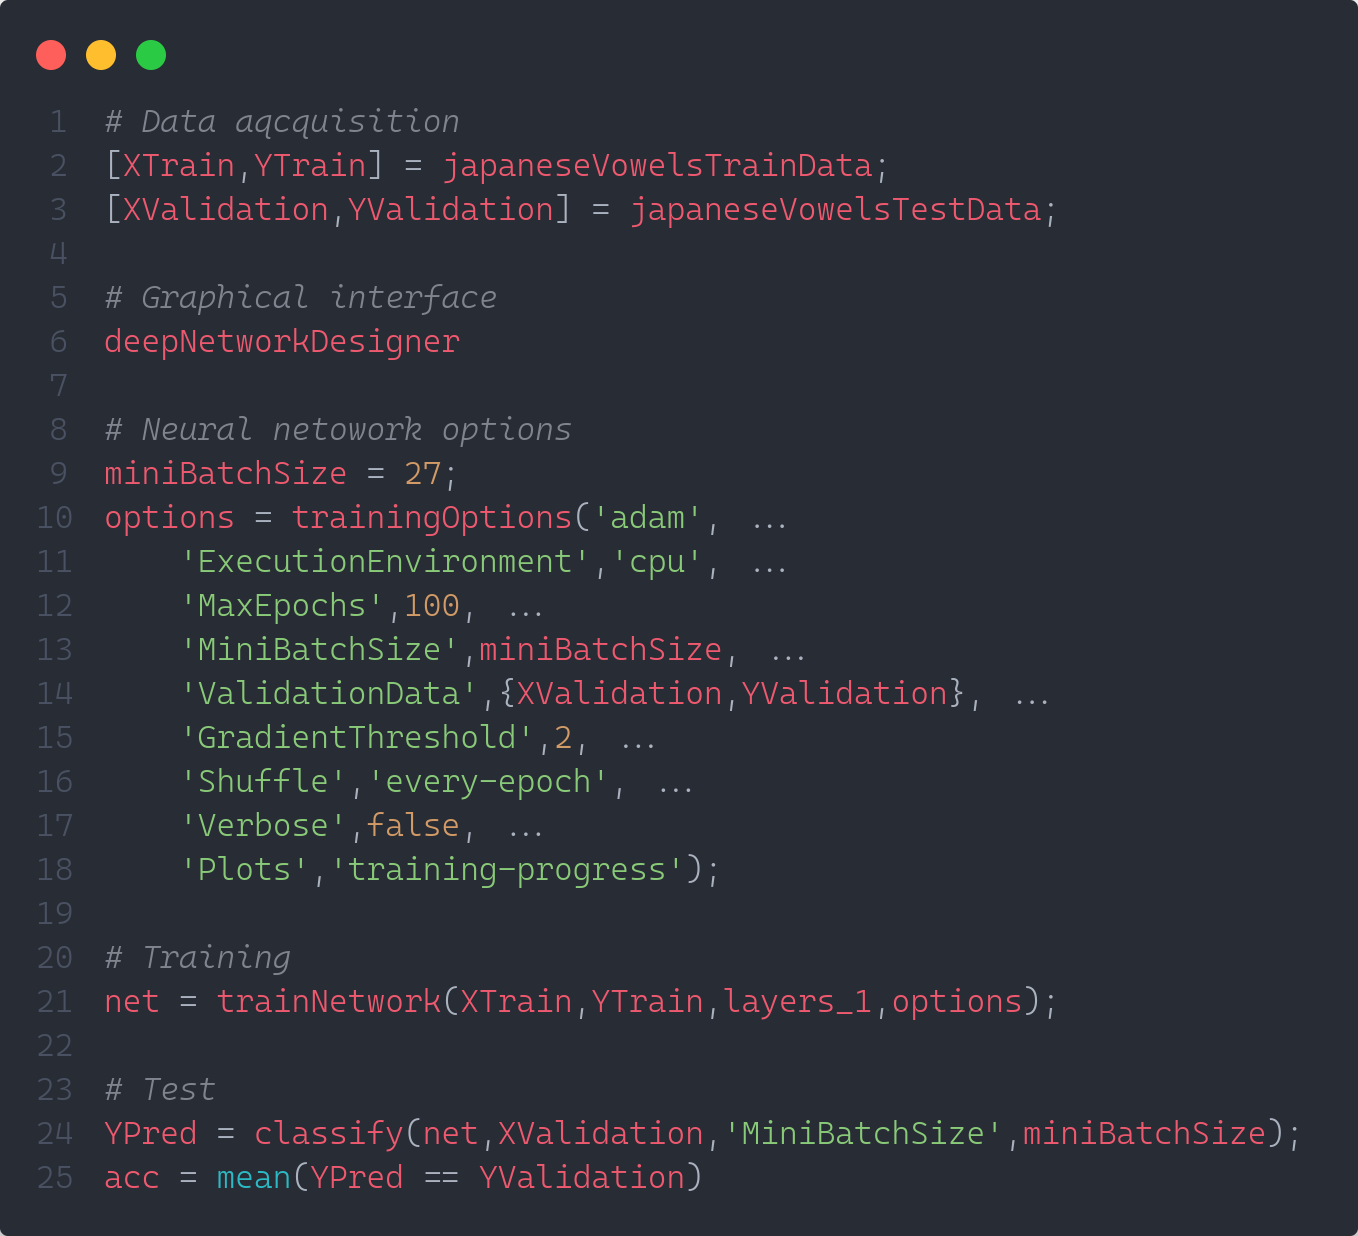
\includegraphics[width=\columnwidth]{figures/nn_code.png}
\end{figure}
\column{0.5\textwidth}
\begin{itemize}
    \item Recurrent Neural Network (RNN).
    \item Vogais do alfabeto japonês.
    \item Flexibilidade para configuração da rede neural.
    \item Precisão: 95,68\%
\end{itemize}
\end{columns}
\end{frame}